In questo capitolo si presenta una sintetica descrizione dei due impianti di depurazione a fanghi attivi della regione Veneto oggetto di studio.


\section{Impianto A}

L'impianto A, come indicato nel Piano di Tutela delle Acque (PTA) della regione Veneto, si trova in una zona omogenea di protezione definita di ricarica degli acquiferi.

Il liquame chiarificato viene scaricato in un fiume e i limiti di emissione sono regolati dalla tabella 1, allegato A, colonna C del PTA. Sebbene a partire dall'8 dicembre 2012 siano entrati in vigore i limiti di emissione per scarico in area sensibile, non si hanno nuove disposizioni poiché la percentuale di riduzione del carico complessivo di azoto totale e fosforo totale in ingresso a tutti gli impianti a livello di bacino è almeno pari al 75\% (art. 25, comma 3 del PTA). Inoltre, nel periodo dell'anno compreso tra aprile e settembre, deve essere rispettato anche il limite per \textit{Escherichia coli}, pari a 5.000 UFC/100 mL \cite{PTA}. La \autoref{tab:sa_limiti} riassume i valori dei limiti indicati dalla normativa sopracitata.

\begin{table}[h]
	\scriptsize
	\begin{center}
		\begin{tabular}{|>{\centering\arraybackslash}p{4cm}|>{\centering\arraybackslash}p{4cm}|>{\centering\arraybackslash}p{4cm}|}
			\hline 
			\textbf{Parametro} & \textbf{Unità di misura} & \textbf{Limite} \\ 
			\hline 
			BOD\textsubscript{5} & mg/L & 25 \\ 
			\hline 
			COD & mg/L & 125 \\ 
			\hline 
			SST & mg/L & 35 \\ 
			\hline 
			P\textsubscript{tot} & mg/L & 10 \\ 
			\hline 
			NH\textsubscript{4}\textsuperscript{+} & mg/L & 15 \\ 
			\hline 
			N-NO\textsubscript{2}\textsuperscript{-} & mg/L & 0,6 \\ 
			\hline 
			N-NO\textsubscript{3}\textsuperscript{-} & mg/L & 20 \\ 
			\hline 
			\textit{E. coli} - da 01/04 a 30/09 & UFC/100 mL & 5.000 \\ 
			\hline 
		\end{tabular} 
		\caption{Limiti allo scarico - impianto A}
		\label{tab:sa_limiti}
	\end{center}	
\end{table}

\subsection{Schema funzionale}
L'impianto, avente una potenzialità autorizzata di 30.000 abitanti equivalenti, è provvisto di una linea acque e di una linea fanghi così strutturate (\autoref{fig:sa_foto} e \autoref{fig:sa_schema}):
\begin{itemize}
	\item Linea acque
		\begin{itemize}
			\item grigliatura grossolana
			\item grigliatura fine - 3 mm (2 linee)
			\item dissabbiatura aerata di tipo pista
			\item equalizzazione e omogeneizzazione
			\item predenitrificazione (3 linee in parallelo)
			\item defosfatazione chimica con cloruro ferrico
			\item sedimentazione secondaria (3 linee in parallelo)
			\item disinfezione finale a raggi U.V.
		\end{itemize}
	\item Linea fanghi
		\begin{itemize}
			\item stabilizzazione aerobica e ispessimento
			\item disidratazione tramite centrifuga
		\end{itemize}
\end{itemize}

In testa all'impianto è posizionato uno sfioratore per le acque meteoriche, dotato di griglia semicilindrica con coclea interna.

\begin{figure}[h]
	\fbox{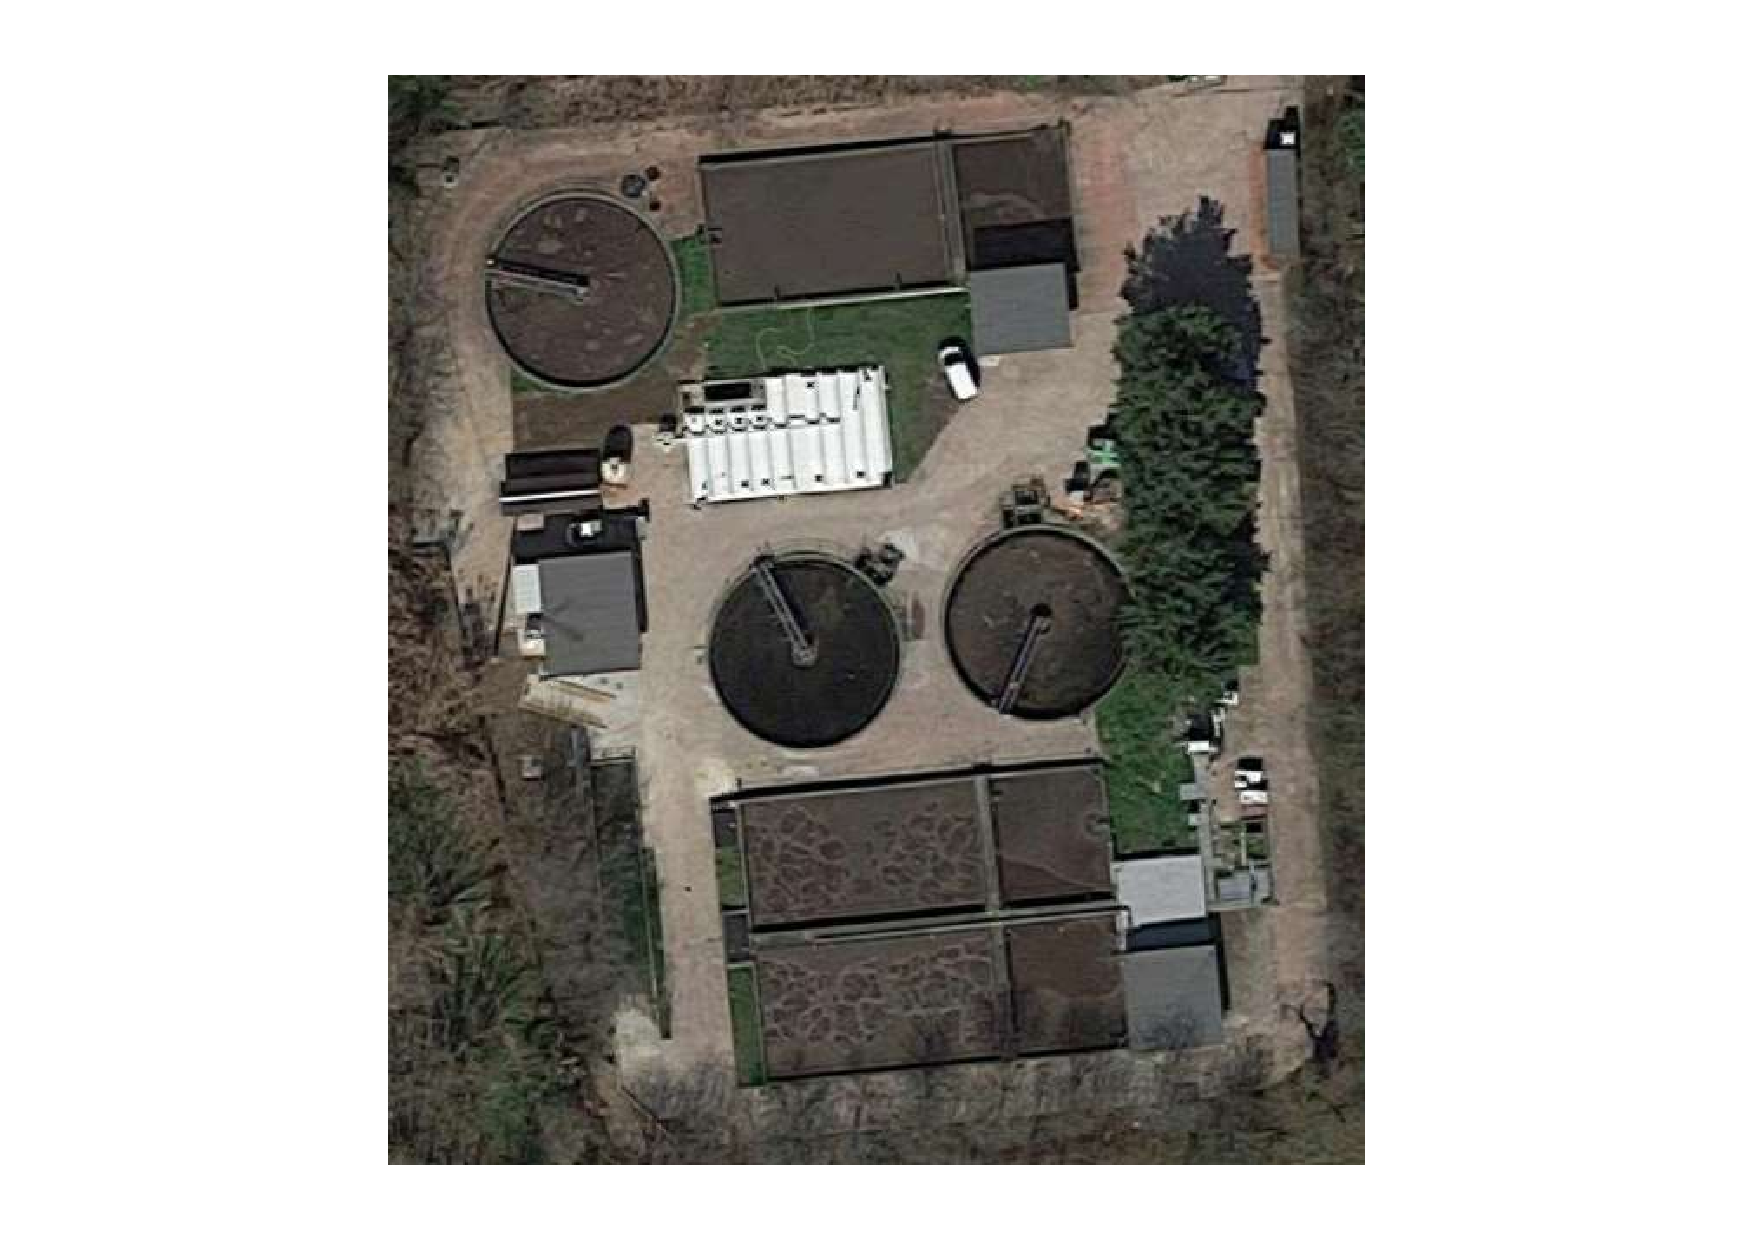
\includegraphics[width=\linewidth]{sa_foto}}	\centering
	\caption{Ripresa aerea dell'impianto A}
	\label{fig:sa_foto}
\end{figure}

\begin{figure}[h]
	\fbox{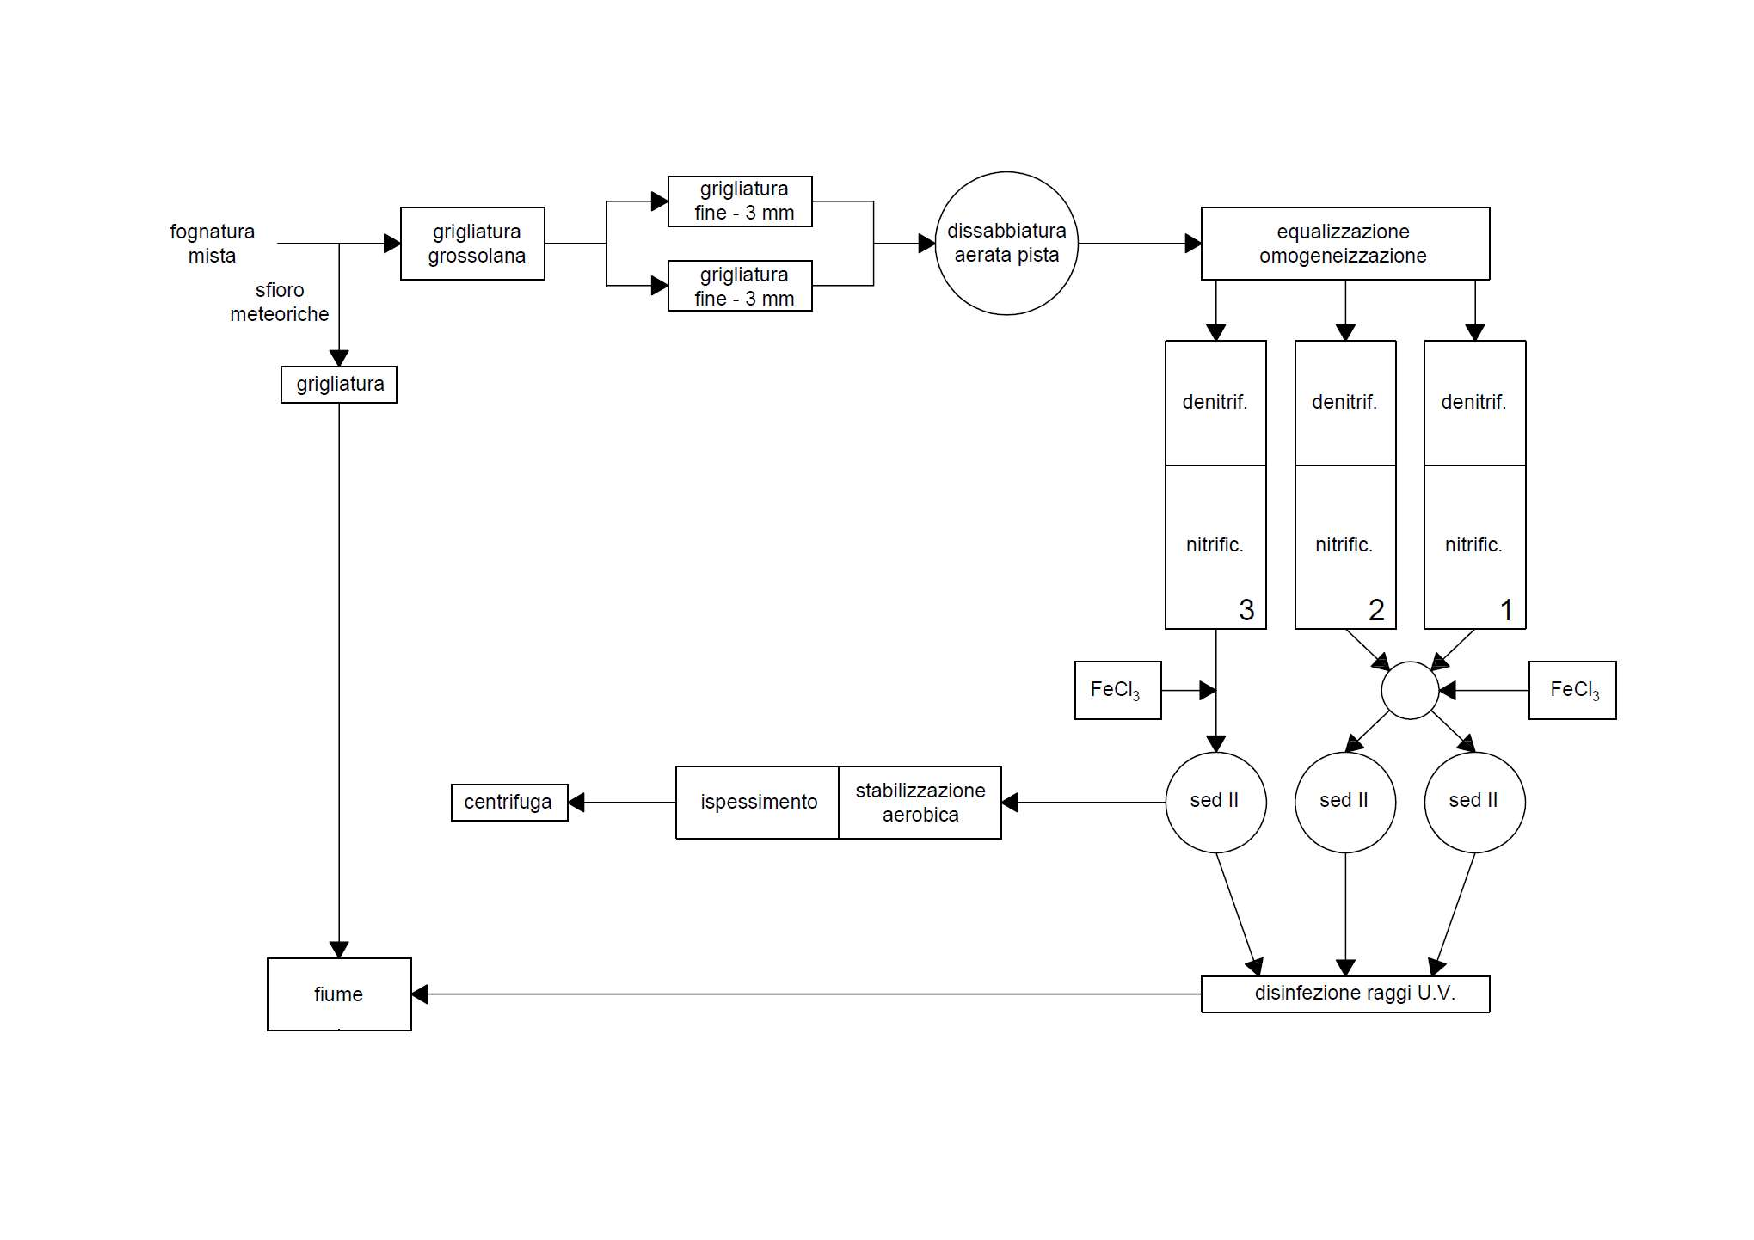
\includegraphics[width=\linewidth]{sa_schema}}	\centering
	\caption{Schema funzionale dell'impianto A}
	\label{fig:sa_schema}
\end{figure}

Relativamente al comparto biologico, si precisa che i processi di denitrificazione e nitrificazione hanno luogo in tre linee parallele. Inoltre, ci sono due circuiti di ricircolo del fango, uno per la nuova linea 3 e uno per le linee 1 e 2, che, quindi, condividono lo stesso fango di ricircolo.

La defosfatazione avviene attraverso il dosaggio di cloruro ferrico per mezzo di due pompe a portata costante: una pompa invia il reattivo alla linea 3 con una certa portata, mentre l'altra invia una portata doppia dello stesso composto alle linee 1 e 2.

Nella linea fanghi, il bacino per la stabilizzazione aerobica è diviso in due parti, entrambe aerate. In una di esse avviene il preispessimento del fango, a monte della centrifugazione dello stesso.

La \autoref{tab:sa_dimensioni} raccoglie i dati dimensionali dei comparti più significativi.

\begin{table}[h]
	\scriptsize
\begin{center}
	\begin{tabular}{|c|l|c|}
		\hline
		\multirow{3}{*}{\textbf{\begin{tabular}[c]{@{}c@{}}Equalizzazione \\ e\\ Omogeneizzazione\end{tabular}}} & Dimensioni in pianta                & 6,8 m x 7,5 m \\
		& Altezza                             & 3,9 m         \\
		& Volume                              & 199 m\textsuperscript{3}        \\ \hline
		\multirow{5}{*}{\textbf{Reattori di ossidazione}}                                                        & Numero                              & 3             \\
		& Dimensioni in pianta                & 10 m x 11,5 m \\
		& Altezza                             & 4,25 m        \\
		& Volume singolo reattore             & 977,5 m\textsuperscript{3}      \\ \cline{2-3} 
		& Volume complessivo                  & 2.932,5 m\textsuperscript{3}    \\ \hline
		\multirow{9}{*}{\textbf{Sedimentatori secondari}}                                                        & Numero                              & 3             \\
		& Diametro                            & 16 m          \\
		& Altezza periferia                   & 2,2 m         \\
		& Area utile singolo sedimentatore   & 185 m\textsuperscript{2}        \\
		& Volume singolo sedimentatore        & 442 m\textsuperscript{3}        \\
		& Circonferenza singolo sedimentatore & 50,24 m       \\ \cline{2-3} 
		& Area complessiva                    & 555 m\textsuperscript{2}        \\
		& Volume complessivo                  & 1.326 m\textsuperscript{3}       \\
		& Circonferenza complessiva           & 150,72 m      \\ \hline
		\textbf{\begin{tabular}[c]{@{}c@{}}Stabilizzazione aerobica \\ e\\ ispessimento\end{tabular}}            & Volume di progetto                  & 680 m\textsuperscript{3}        \\ \hline
	\end{tabular}
	\caption{Dati dimensionali dei principali comparti dell'impianto A}
	\label{tab:sa_dimensioni}
\end{center}
\end{table}


\subsection{Dotazioni}
In \autoref{tab:sa_vinc-idr} si riportano alcuni vincoli idraulici, estratti dalla documentazione di progetto.

\begin{table}
	\scriptsize
\begin{center}
	\begin{tabular}{|l|c|}
		\hline
		\textbf{\begin{tabular}[c]{@{}l@{}}Portata massima in tempo di pioggia \\ (da collaudo funzionale)\end{tabular}}  & \begin{tabular}[c]{@{}c@{}}Totale: 499,8 m\textsuperscript{3}/h\\ Ciascuna linea: 166,6 m\textsuperscript{3}/h\end{tabular} \\ \hline
		\textbf{Portata massima disinfezione a raggi U.V.}                                                                & 500 m\textsuperscript{3}/h                                                                                \\ \hline
		\textbf{Portata massima dissabbiatore di tipo pista}                                                              & 648 m\textsuperscript{3}/h                                                                                \\ \hline
		\textbf{\begin{tabular}[c]{@{}l@{}}Portata e carico massimi centrifuga \\ per disidratazione fanghi\end{tabular}} & 9 m\textsuperscript{3}/h, 180 kgSS/h                                                                      \\ \hline
	\end{tabular}
	\caption{Vincoli idraulici}
	\label{tab:sa_vinc-idr}
\end{center}
\end{table}


Il comparto di ossidazione/nitrificazione è aerato tramite un totale di quattro elettrosoffianti Robuschi: due sono a servizio delle vecchie linee (linea 1 e linea 2), uno è a servizio della nuova linea (linea 3) e uno è di riserva. Le loro caratteristiche sono riassunte in \autoref{tab:sa_elettrosoffiatori}.

Ipotizzando che in aspirazione l'aria abbia una temperatura di 30\textdegree C e una pressione di 1 atm, la portata totale insufflabile è di circa 4.400 Nm\textsuperscript{3}/h (1.100 Nm\textsuperscript{3}/h per ogni singolo compressore). La logica di funzionamento dei compressori è basata su un valore di set point di 2 mg/L.

Il surnatante proveniente dall'ispessitore viene ricircolato a metà della vasca di ossidazione della linea 3, mentre il centrato viene immesso all'uscita della medesima vasca.\\

\begin{table}
	\scriptsize
\begin{center}
	\begin{tabular}{|c|l|c|}
		\hline
		\multicolumn{3}{|c|}{\textbf{Linee 1 e 2}}                                                                                                                   \\ \hline
		\multirow{3}{*}{\textbf{\begin{tabular}[c]{@{}c@{}}Compressore tipo ES 85/3P - RVP125\\ (inverter)\end{tabular}}}   & Portata aspirazione {[}m\textsuperscript{3}/h{]} & 1.225 \\
		& $\Delta$p {[}mbar{]}                  & 450   \\
		& rpm {[}min\textsuperscript{-1}{]}                  & 2.081 \\ \hline
		\multirow{3}{*}{\textbf{\begin{tabular}[c]{@{}c@{}}Compressore tipo ES 86/3P - RVP125\\ (soft-start)\end{tabular}}} & Portata aspirazione {[}m\textsuperscript{3}/h{]} & 1.213 \\
		& $\Delta$p {[}mbar{]}                  & 450   \\
		& rpm {[}min\textsuperscript{-1}{]}                  & 1.670 \\ \hline
		\multicolumn{3}{|c|}{\textbf{Linea 3}}                                                                                                                       \\ \hline
		\multirow{3}{*}{\textbf{\begin{tabular}[c]{@{}c@{}}Compressore tipo ES 85/3P - RVP125\\ (soft-start)\end{tabular}}} & Portata aspirazione {[}m\textsuperscript{3}/h{]} & 1.225 \\
		& $\Delta$p {[}mbar{]}                  & 450   \\
		& rpm {[}min\textsuperscript{-1}{]}                  & 2.081 \\ \hline
		\multirow{3}{*}{\textbf{\begin{tabular}[c]{@{}c@{}}Compressore tipo ES 86/3P - RVP125\\ (riserva)\end{tabular}}}    & Portata aspirazione {[}m\textsuperscript{3}/h{]} & 1.213 \\
		& $\Delta$p {[}mbar{]}                  & 450   \\
		& rpm {[}min\textsuperscript{-1}{]}                   & 1.670 \\ \hline
	\end{tabular}
	\caption{Caratteristiche degli elettrosoffianti}
	\label{tab:sa_elettrosoffiatori}
\end{center}
\end{table}

La strumentazione presente all'interno dell'impianto consiste in:
\begin{itemize}
	\item autocampionatori, uno all'ingresso (dopo la grigliatura) e uno all'uscita, funzionanti in base alla portata;
	\item torbidimetro all'uscita finale;
	\item misuratore di portata a ultrasuoni sul canale di alimentazione alla dissabbiatura;
	\item sonde per l'ossigeno disciolto, una all'uscita delle linee 1 e 2 e una sulla linea 3;
	\item misuratore di livello ad ultrasuoni sul comparto di stabilizzazione aerobica per la misura della quantità di fango estratta dal comparto biologico;
	\item pH-metro in equalizzazione.
\end{itemize}
Ad eslusione di torbidimetro e pH-metro, gli strumenti sono dotati di \textit{data logger} per la memorizzazione delle misure.

\clearpage
\section{Impianto B}
L'impianto B, come indicato nel Piano di Tutela delle Acque (PTA) della regione Veneto, è collocato in una zona omogenea di protezione definita come zona montana.

L'effluente viene immesso in due torrenti successivi e i limiti di emissione sono regolati dalla tabella 1, allegato A, colonna C del PTA, ma per i parametri BOD\textsubscript{5}, COD, azoto totale e fosforo totale si devono rispettare i limiti di tabella 4, allegato 5, parte III del D. Lgs. 152/06 relativa allo scarico sul suolo \cite{PTA} \cite{DLgs152}. Questo è giustificato dal fatto che i corpi idrici ricettori sono a carattere torrentizio, ovvero, in tempo secco, hanno una portata praticamente nulla. In particolare, per quanto riguarda i limiti imposti per azoto totale e fosforo totale, si precisa che, sebbene numericamente siano coincidenti con i limiti per scarico in area sensibile, essi sono da considerarsi come valori puntuali e non come media annua (come quelli per scarico in area sensibile). Il limite per \textit{Escherichia coli}, fissato dall'autorità competente in fase di autorizzazione allo scarico, tenendo conto delle condizioni ambientale e igienico-sanitaria del corpo idrico ricettore, è pari a 5.000 UFC/100 mL. La \autoref{tab:c_limiti} riassume i valori dei limiti indicati dalla normativa sopracitata.

\begin{table}[h]
	\scriptsize
	\begin{center}
		\begin{tabular}{|>{\centering\arraybackslash}p{4cm}|>{\centering\arraybackslash}p{4cm}|>{\centering\arraybackslash}p{4cm}|}
			\hline 
			\textbf{Parametro} & \textbf{Unità di misura} & \textbf{Limite} \\ 
			\hline 
			BOD\textsubscript{5} & mg/L & 20 \\ 
			\hline 
			COD & mg/L & 100 \\ 
			\hline 
			SST & mg/L & 35 \\ 
			\hline 
			P\textsubscript{tot} & mg/L & 2 \\ 
			\hline 
			N\textsubscript{tot} & mg/L & 15 \\ 
			\hline 
			NH\textsubscript{4}\textsuperscript{+} & mg/L & 15 \\ 
			\hline 
			N-NO\textsubscript{2}\textsuperscript{-} & mg/L & 0,6 \\ 
			\hline 
			N-NO\textsubscript{3}\textsuperscript{-} & mg/L & 20 \\ 
			\hline 
			\textit{E. coli} & UFC/100 mL & 5.000 \\
			\hline
		\end{tabular} 
		\caption{Limiti allo scarico - impianto B}
		\label{tab:c_limiti}
	\end{center}	
\end{table}

\subsection{Schema funzionale}
L'impianto, avente una potenzialità autorizzata di 10.000 abitanti equivalenti e dimensionato per una portata di 2.000 m\textsuperscript{3}/d, è provvisto di una linea acque e di una linea fanghi così strutturate (\autoref{fig:c_foto} e \autoref{fig:c_schema}):
\begin{itemize}
	\item Linea acque
	\begin{itemize}
		\item grigliatura - 3 mm
		\item dissabbiatura aerata
		\item equalizzazione aerata
		\item equalizzazione
		\item denitrificazione
		\item nitrificazione (2 linee)
		\item defosfatazione chimica con policloruro di alluminio
		\item sedimentazione secondaria
		\item disinfezione chimica
	\end{itemize}
	\item Linea fanghi
	\begin{itemize}
		\item stabilizzazione aerobica, con possibilità di ispessimento (3 bacini)
		\item disidratazione tramite centrifuga mobile
	\end{itemize}
\end{itemize}

\begin{figure}[h]
	\fbox{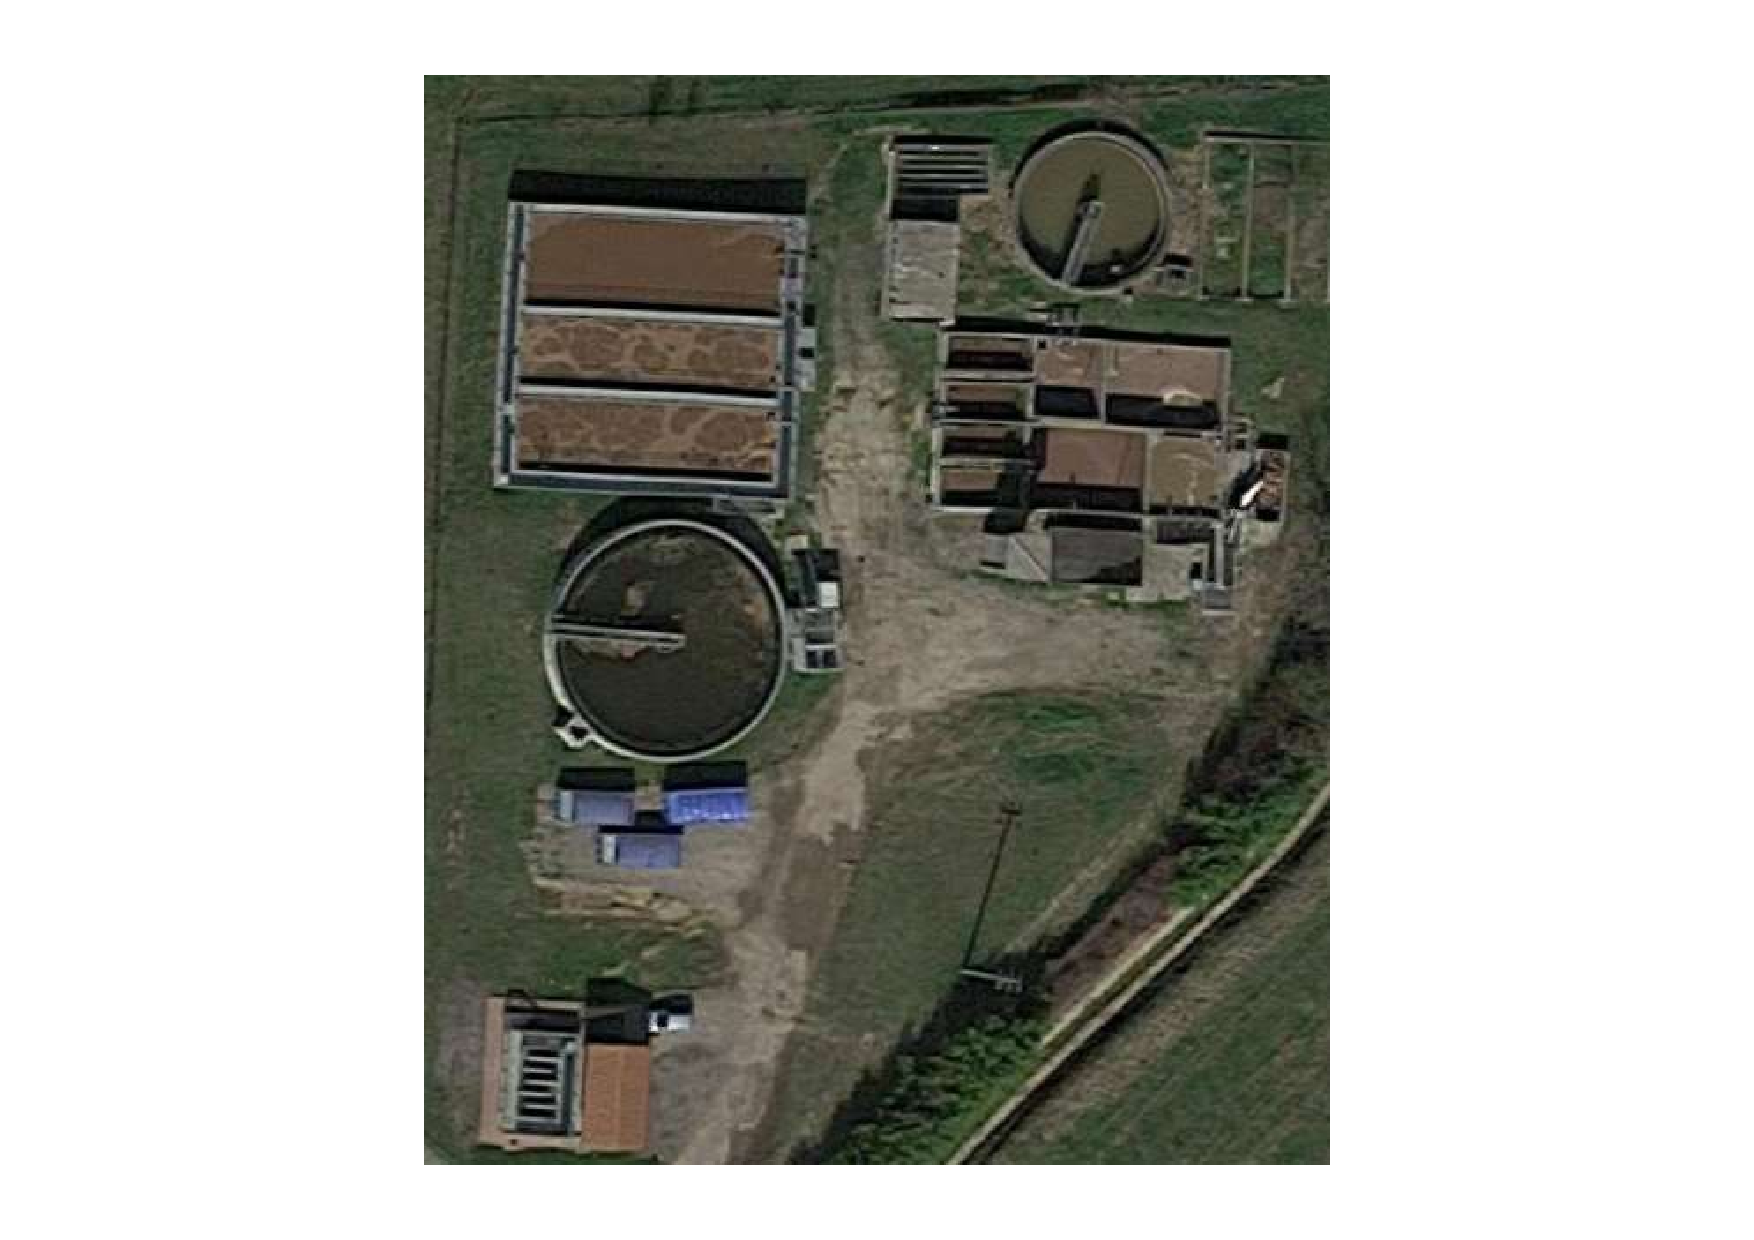
\includegraphics[width=\linewidth]{c_foto}}	\centering
	\caption{Ripresa aerea dell'impianto B}
	\label{fig:c_foto}
\end{figure}
\begin{figure}[h]
	\fbox{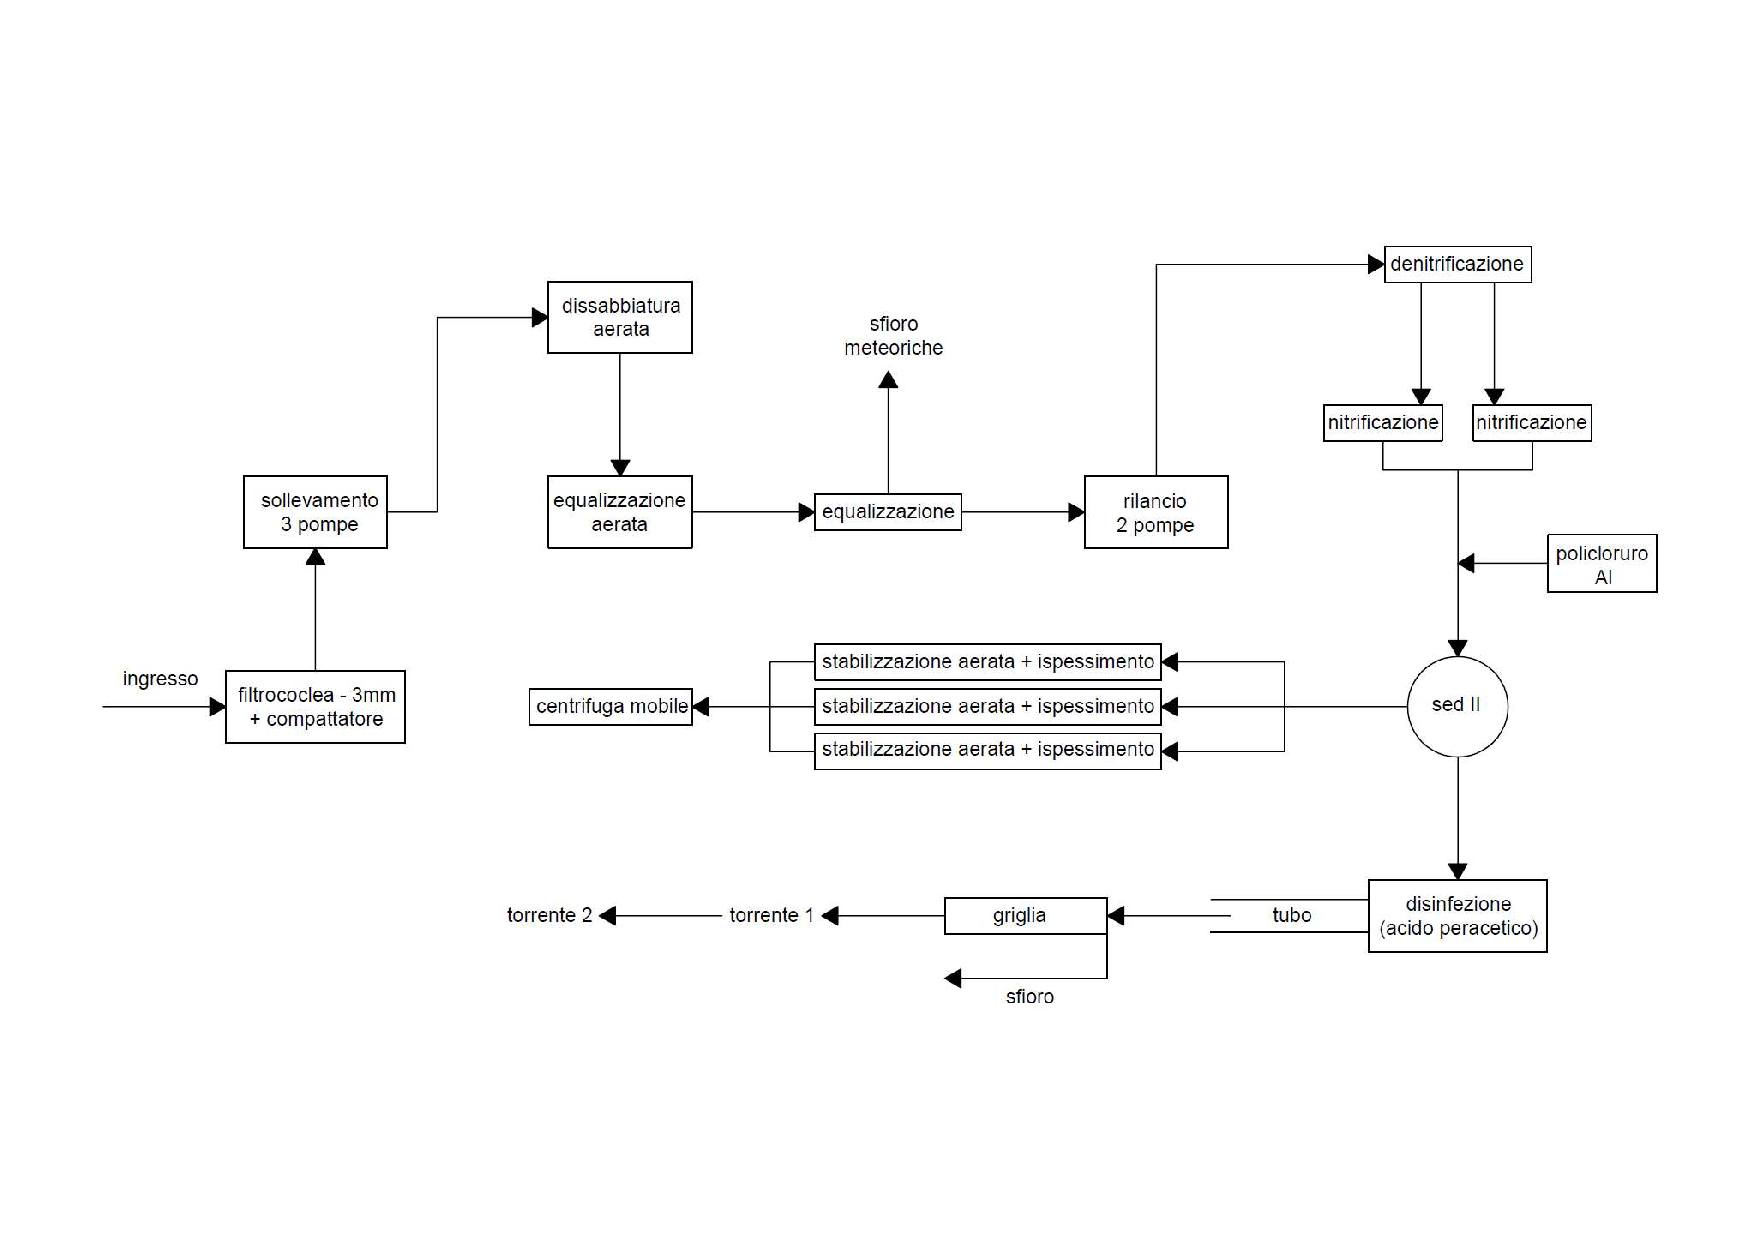
\includegraphics[width=\linewidth]{c_schema}}	\centering
	\caption{Schema funzionale dell'impianto B}
	\label{fig:c_schema}
\end{figure}

Il comparto di equalizzazione è provvisto di uno sfioro che, in tempo di pioggia, invia le acque miste a una linea di trattamento costituita da sedimentazione e disinfezione.

Relativamente alla disinfezione, l'acido peracetico non viene dosato nel comparto di disinfezione stesso, bensì nel rispettivo canale di by-pass.

A seguito della disinfezione finale, il refluo viene convogliato, attraverso una tubazione interrata, a un manufatto di grigliatura che successivamente scarica nei corpi idrici ricettori.

In \autoref{tab:c_dimensioni} sono raccolti i dati dimensionali dei comparti più significativi.


\begin{table}
	\scriptsize
\begin{center}
	\begin{tabular}{|c|l|c|}
		\hline
		\multirow{3}{*}{\textbf{Dissabbiatura aerata}}                                                                                                    & Dimensioni in pianta          & 6,6 m x 4,4 m \\
		& Altezza                       & 3,25 m        \\
		& Volume                        & 94,38 m\textsuperscript{3}      \\ \hline
		\multirow{3}{*}{\textbf{\begin{tabular}[c]{@{}c@{}}Equalizzazione (dimensione \\ totale dei due bacini \\ idraulicamente collegati)\end{tabular}}} & Dimensioni in pianta          & 15 m x 6,6 m  \\
		& Altezza                       & 5 m           \\
		& Volume                        & 495 m\textsuperscript{3}        \\ \hline
		\multirow{3}{*}{\textbf{Reattore di denitrificazione}}                                                                                            & Dimensioni in pianta          & 20 m x 8 m    \\
		& Altezza                       & 4,25 m        \\
		& Volume                        & 680 m\textsuperscript{3}        \\ \hline
		\multirow{5}{*}{\textbf{Reattori di ossidazione}}                                                                                                 & Numero                        & 2             \\
		& Dimensioni in pianta          & 20 m x 5,8 m  \\
		& Altezza                       & 4,25 m        \\
		& Volume singolo reattore       & 493 m\textsuperscript{3}       \\ \cline{2-3} 
		& Volume complessivo            & 986 m\textsuperscript{3}        \\ \hline
		\multirow{5}{*}{\textbf{Sedimentatore secondario}}                                                                                                & Diametro utile                & 18 m          \\
		& Altezza periferia             & 2,6 m         \\
		& Area                          & 254 m\textsuperscript{2}        \\
		& Volume                        & 762 m\textsuperscript{3}        \\
		& Circonferenza                 & 56,5 m        \\ \hline
		\multirow{3}{*}{\textbf{Vasca di disinfezione}}                                                                                                   & Dimensioni in pianta          & 5,2 m x 3 m   \\
		& Altezza                       & 2,25 m        \\
		& Volume                        & 35,1 m\textsuperscript{3}       \\ \hline
		\multirow{9}{*}{\textbf{\begin{tabular}[c]{@{}c@{}}Stabilizzazione aerata\\ e\\ ispessimento\end{tabular}}}                                       & Numero                        & 2             \\
		& Dimensioni in pianta          & 6 m x 6 m     \\
		& Altezza                       & 4 m           \\
		& Volume singolo bacino         & 144 m\textsuperscript{3}        \\ \cline{2-3} 
		& Numero                        & 1             \\
		& Dimensioni in pianta          & 10 m x 6 m    \\
		& Altezza                       & 4 m           \\
		& Volume                        & 240 m\textsuperscript{3}        \\ \cline{2-3} 
		& Volume complessivo (3 bacini) & 528 m\textsuperscript{3}        \\ \hline
	\end{tabular}
	\caption{Dati dimensionali dei principali comparti dell'impianto B}
	\label{tab:c_dimensioni}
\end{center}
\end{table}

\subsection{Dotazioni}

La \autoref{tab:c_macchinari} riporta le caratteristiche delle principali attrezzature elettromeccaniche presenti all'interno dell'impianto.

La logica di automazione dell'impianto prevede un'alimentazione a portata costante (circa 85 m\textsuperscript{3}/h). Le pompe per il rilancio del liquame dalla vasca di equalizzazione a quella di denitrificazione si avviano e si arrestano in funzione del livello nella vasca di equalizzazione.

Per l'aerazione della vasca di ossidazione, se si ipotizza che l'aria in aspirazione abbia una temperatura pari a 30\textdegree C, la portata di aspirazione corrisponde a circa 1.550 Nm\textsuperscript{3}/h. Le due elettrosoffianti sono dotate di inverter che lavorano in funzione della concentrazione di ossigeno disciolto in vasca di ossidazione, il cui set point è di 1 mg/L.

Il surnatante dell'ispessitore è ricircolato a valle del sollevamento e del campionatore di portata, mentre il ricircolo del centrato è immesso all'inizio del comparto di denitrificazione.\\

La strumentazione presente all'interno dell'impianto consiste in:
\begin{itemize}
	\item autocampionatori, uno all'ingresso (prima della dissabbiatura) e uno all'uscita;
	\item misuratore di portata ad induzione elettromagnetica installato sull'alimentazione del comparto biologico;
	\item misuratore di portata a ultrasuoni (rileva la misura del battente su uno stramazzo in parete sottile) installato allo scarico;
	\item sonda per la misura dell'ossigeno disciolto nella vasca di ossidazione.
\end{itemize}

Tutti questi strumenti sono dotati di \textit{data logger} per la memorizzazione delle misure.	\\

\begin{table}[!h]
	\scriptsize
	\begin{center}
		\begin{tabular}{|c|l|c|}
			\hline
			\multicolumn{3}{|c|}{\textbf{Grigliatura}}                                                                                                                                        \\ \hline
			\multirow{3}{*}{\textbf{\begin{tabular}[c]{@{}c@{}}Filtrococlea \\ SAVI VSR-700\end{tabular}}}                                           & Luce di filtrazione {[}mm{]}   & 3     \\
			& Portata massima {[}L/s{]}      & 160   \\
			& Portata massima {[}m\textsuperscript{3}/h{]}     & 576   \\ \hline
			\multicolumn{3}{|c|}{\textbf{Rilancio equalizzazione - denitrificazione}}                                                                                                         \\ \hline
			\multirow{4}{*}{\textbf{Pompe}}                                                                                                          & Numero                         & 2     \\
			& Portata massima {[}L/s{]}      & 26    \\
			& Portata massima {[}m\textsuperscript{3}/d{]}     & 2.246 \\
			& Prevalenza massima {[}m{]}     & 7,2   \\ \hline
			\multicolumn{3}{|c|}{\textbf{Ricircolo del fango}}                                                                                                                                \\ \hline
			\multirow{3}{*}{\textbf{Pompe}}                                                                                                          & Numero                         & 2     \\
			& Portata massima {[}L/s{]}      & 27    \\
			& Prevalenza massima {[}m{]}     & 3     \\ \hline
			\multicolumn{3}{|c|}{\textbf{Aerazione ossidazione}}                                                                                                                              \\ \hline
			\multirow{4}{*}{\textbf{\begin{tabular}[c]{@{}c@{}}Elettrosoffiante Rocuschi Robox\\ tipo ES 85/3P - RVP125\\ (inverter)\end{tabular}}} & Numero                         & 2     \\
			& Portata aspirazione {[}m\textsuperscript{3}/h{]} & 1.711 \\
			& $\Delta$p {[}mbar{]}                  & 530   \\
			& rpm {[}min\textsuperscript{-1}{]}                  & 2.792 \\ \hline
		\end{tabular}
		\caption{Caratteristiche delle principali apparecchiature elettromeccaniche}
		\label{tab:c_macchinari}
	\end{center}
\end{table}


